\documentclass[UTF8]{ctexart}
\usepackage{ctex}                   % 支持中文
\usepackage{amsmath,amssymb}        % 支持数学公式
\usepackage{geometry}               % 排版页边距
\usepackage{pifont}                 % 带圈的数字
\usepackage{extarrows}              % 支持x箭头系列
\usepackage{mathrsfs}               % 支持大写花体字母
\usepackage{color}                  % 支持颜色
\usepackage{multirow}               % 支持合并单元格
\usepackage{graphicx}               % 支持插图
\usepackage{esint}                  % 支持环路积分符号
\usepackage{multicol}               % 支持分栏
\usepackage{listings}               % 支持代码块
\usepackage{fancyhdr}               % 设置页眉页脚
\usepackage{xcolor}
\usepackage{enumerate}
\usepackage{enumitem}
\usepackage{subfigure}              % 支持子图
\usepackage{caption}

% 清除页眉,保留页脚的页码编号
\pagestyle{plain}
% 更改页边距
\geometry{left=19.1mm,right=19.1mm,top=25.4mm,bottom=25.4mm}
% 更改section的自动编号方式
\renewcommand\thesection{\zhnum{section}}
\renewcommand\thesubsection{\arabic{section}.\arabic{subsection}}
% 更改公式自动编号的方式
\renewcommand{\theequation}{\arabic{section}.\arabic{equation}}
% 代码块设置
\definecolor{mygreen}{rgb}{0,0.6,0}
\setmonofont{Consolas}
\lstset{language = matlab, numbers=left,
    breaklines=true, frame=single, numbersep=5pt,
    showspaces=false,
    columns=fullflexible,
    numberstyle=\tiny, keywordstyle=\color{blue!70},
    commentstyle=\color{mygreen},
    rulesepcolor=\color{red!0!green!0!blue!0}, basicstyle=\ttfamily,
    xleftmargin=1em, xrightmargin=1em, aboveskip=1em
}
% 一个单元格内的内容自动换行
\newcommand{\tabincell}[2]{\begin{tabular}{@{}#1@{}}#2\end{tabular}}
% 修改摘要的标题大小
% \renewcommand{\abstractname}{\large 摘要\\}
\title{\heiti 维纳滤波与约束最小二乘方滤波图像复原的介绍与比较}
\author{}
\date{}

\begin{document}
    \maketitle
    \textbf{关键词}:噪声,维纳滤波,约束最小二乘方滤波,图像复原,Matlab
    \section{两种图像复原方法的理论介绍}
    \subsection{引言:图像复原}
    在图像生成、记录、传输过程中,由于成像系统、设备或外在的干扰,会导致图像质量下降,这种现象称为图像退化。如,大气扰动效应、光学系统的像差、物体运动造成的模糊、几何失真等。对退化图像进行处理,使之恢复原貌的技术称之为图像复原(Image Restoration)。

    图像复原的关键在于确定退化的相关知识,将退化过程模型化,采用相反的过程尽可能地恢复原图,或者说使复原后的图像尽可能地接近原图。

    用简单的语言来说,就是恢复图像本来的面貌,但由于各种原因如图像采集过程中出现的误差导致得到的数字图像不清晰,不是我们人眼看到的实物场景那样,因此需要采取技术手段去除图像的不清晰。在本文中会介绍两种较常用的图像复原方法——维纳滤波与约束最小二乘方滤波。
    \subsection{利用维纳滤波进行图像复原}
    在日常生活中,我们所拍摄的对象时常不会处于完全静止的状态,而由于其运动,所拍摄的照片会产生许多噪声。但是用一些简单的逆滤波方法不能很好地处理噪声需要采用约束复原的方法,维纳滤波(最小均方误差滤波器)复原就是一种有代表性的约束复原方法,是使原始图像$f(x,y)$和复原图像$\hat{f}(x,y)$之间均方误差最小的复原方法。

    均方误差的表达式为:
    \begin{equation}
        e^2=E\left[(f-\hat{f})^2\right]
    \end{equation}

    假设噪声$n(x,y)$和图像$f(x,y)$不相关,且$f(x,y)$或$n(x,y)$有零均值,估计的灰度级$\hat{f}(x,y)$是退化图像灰度级$g(x,y)$的线性函数,在这些条件下,当均方误差取最小值时有下列表达式

    \begin{equation}\label{eqsetmin}
    \begin{split}
        \hat{F}(u,v)&=\left[\frac{H^*(u,v)S_f(u,v)}{S_f(u,v)|H(u,v)|^2+S_n(u,v)}\right]G(u,v)\\
        &=\left[\frac{H^*(u,v)}{|H(u,v)|^2+S_n(u,v)/S_f(u,v)}\right]G(u,v)\\
        &=\left[\frac{1}{H(u,v)}\cdot\frac{|H(u,v)|^2}{|H(u,v)|^2+S_n(u,v)/S_f(u,v)}\right]G(u,v)
    \end{split}
    \end{equation}
    式中,$H^*(u,v)$是退化函数$H(u,v)$的复共轭;$S_n(u,v)=|N(u,v)|^2$是噪声的功率谱;$S_f(u,v)=|F(u,v)|^2$是原图的功率谱。

    由式(\ref{eqsetmin})可以看出,维纳滤波器的传递函数为
    \begin{equation}
        H_w(u,v)=\frac{1}{H(u,v)}\cdot\frac{|H(u,v)|^2}{|H(u,v)|^2+S_n(u,v)/S_f(u,v)}
    \end{equation}

    从式(\ref{eqsetmin})中可以看出,维纳滤波器没有逆滤波(也是一种图像复原方法)中传递函数为零的问题,除非对于相同的$u,v$值,$H(u,v)$和$S_n(u,v)$同时为零。因此,维纳滤波能够自动抑制噪声。

    当噪声为零时,噪声功率谱小,维纳滤波变成了逆滤波,因此,逆滤波是维纳滤波的特例。当$S_n(u,v)$远大于$S_f(u,v)$时,则$H_w(u,v) \to 0$,维纳滤波器避免了逆滤波过于放大噪声的问题。

    采用维纳滤波器复原图像时,需要知道原始图像和噪声的功率谱$S_f(u,v)$和$S_n(u,v)$,而实际上这些值是未知的,通常采用一个常数$K$来代替$\displaystyle\frac{S_n(u,v)}{S_f(u,v)}$,即使用式(\ref{eqabout})来近似表达:
    \begin{equation}\label{eqabout}
        \hat{F}(u,v)=\left[\frac{1}{H(u,v)}\cdot\frac{|H(u,v)|^2}{|H(u,v)|^2+K}\right]G(u,v)
    \end{equation}

    \subsection{利用约束最小二乘方滤波进行图像处理}
    \subsubsection{约束最小二乘方滤波的原理}
    对原图像进行某一线性运算$Q$,约束复原就是求在约束条件$||\pmb{n}||^2=||\pmb{g}-\pmb{H}\hat{\pmb{f}}||^2$下,使$||\pmb{Q}\hat{\pmb{f}}||^2$为最小的原图$\pmb{f}$的最佳估计$\hat{\pmb{f}}$。在此,在使用最小化原图二阶微分的方法前,先使用拉格朗日乘数法导出约束复原结论(后文会用到)。

    构造拉格朗日函数
    \begin{equation}\label{eqlagrange}
        J(\hat{\pmb{f}})=||\pmb{Q}\hat{\pmb{f}}||^2+\lambda\left(||\pmb{g}-\pmb{H}\hat{\pmb{f}}||^2-||\pmb{n}||^2\right)
    \end{equation}
    式中,$\lambda$为拉格朗日系数。

    将式(\ref{eqlagrange})求微分以最小值:
    \begin{equation}
        \frac{\partial J\left(\hat{\pmb{f}}\right)}{\partial \hat{\pmb{f}}}=2\pmb{Q}^{\mathrm{T}}\pmb{Q}\hat{\pmb{f}}+2\lambda\pmb{H}^{\mathrm{T}}\left(\pmb{g}-\pmb{H}\hat{\pmb{f}}\right)=0
    \end{equation}

    求解:
    \[\pmb{Q}^{\mathrm{T}}\pmb{Q}\hat{\pmb{f}}+\lambda\pmb{H}^{\mathrm{T}}\pmb{H}\hat{\pmb{f}}-\lambda\pmb{H}^{\mathrm{T}}\pmb{g}=0\]
    \[\frac{1}{\lambda}\pmb{Q}^{\mathrm{T}}\pmb{Q}\hat{\pmb{f}}+\pmb{H}^{\mathrm{T}}\pmb{H}\hat{\pmb{f}}=\pmb{H}^{\mathrm{T}}\pmb{g}\]
    \begin{equation}\label{eqlimitbackcon}
        \hat{\pmb{f}}=\left(\pmb{H}^{\mathrm{T}}\pmb{H}+\frac{1}{\lambda}\pmb{Q}^{\mathrm{T}}\pmb{Q}\right)^{-1}+\pmb{H}^{\mathrm{T}}\pmb{g}
    \end{equation}
    式(\ref{eqlimitbackcon})就是约束复原结论。

    现在,开始使用最小化原图二阶微分的方法,图像$f(x,y)$在$(x,y)$处的二阶微分可表示为
    \begin{equation}
        \nabla^2 f=\frac{\partial^2 f}{\partial x^2}+\frac{\partial^2 f}{\partial y^2}=f(x+1,y)+f(x-1,y)+f(x,y+1)+f(x,y-1)-4f(x,y)
    \end{equation}

    二阶微分实际上是原图$f(x,y)$与离散的拉普拉斯算子$\pmb{l}(x,y)$的卷积:
    \begin{equation}
        l(x,y)=\left(\begin{array}{ccc}
            \begin{matrix}
                0 & 1 & 0\\1 & -4 &1\\0 & 1 & 0
            \end{matrix}
        \end{array}\right)
    \end{equation}

    采取的最优化准则为:
    \begin{equation}
        \min\left\{f(x,y)*l(x,y)\right\}
    \end{equation}

    拉普拉斯算子尺寸为$3 \times 3$,设原图像大小为$A \times B$,系统函数$H$大小为$C \times D$,为避免折叠现象,将各函数延拓到$M \times N,M \geq A+C-1$且$M \geq A+3-1$;$N \geq B+D-1$且$N \geq B+3-1$,即:
    \begin{equation}\label{eq1ddef}
    \begin{split}
        f_e(x,y)&=\begin{cases}
            f(x,y) & 0 \leq x \leq A-1,0 \leq y \leq B-1\\0 & A \leq x \leq M-1,B \leq y \leq N-1
        \end{cases}\\
        h_e(x,y)&=\begin{cases}
            h(x,y) & 0 \leq x \leq C-1,0 \leq y \leq D-1\\0 & C \leq x \leq M-1,D \leq y \leq N-1
        \end{cases}\\
        l_e(x,y)&=\begin{cases}
            l(x,y) & 0 \leq x \leq 2,0 \leq y \leq 2\\0 & 3 \leq x \leq M-1,3 \leq y \leq N-1
        \end{cases}\\
        g_e(x,y)&=\begin{cases}
            g(x,y) & 0 \leq x \leq A+C-2,0 \leq y \leq B+D-2\\0 & A+C-1 \leq x \leq M-1,B+D-1 \leq y \leq N-1
        \end{cases}\\
    \end{split}
    \end{equation}

    原图$\pmb{f}(x,y)$与拉普拉斯算子$l(x,y)$的卷积表达为矩阵形式:
    \begin{equation}
        \pmb{Lf}=\left(\begin{array}{cccc}
            \begin{matrix}
                L_0 & L_{M-1} & \cdots & L_1\\L_1 & L_0 & \cdots & L_2\\\vdots & \vdots & & \vdots\\L_{M-1} & L_{M-2} & \cdots & L_0
            \end{matrix}
        \end{array}\right)\left(\begin{array}{c}
            \begin{matrix}
                f_e(0)\\f_e(1)\\\vdots\\f_e(MN-1)
            \end{matrix}
        \end{array}\right)
    \end{equation}
    其中,$\pmb{L}$的每个部分$\pmb{L}_j$都是一个循环阵,由延拓函数$l_e(x,y)$的第$j$列构成:
    \begin{equation}
        \pmb{L}_j=\left(\begin{array}{cccc}
            \begin{matrix}
                l_e(j,0) & l_e(j,N-1) & \cdots & l_e(j,1)\\l_e(j,1) & l_e(j,0) & \cdots & l_e(j,2)\\\vdots & \vdots & & \vdots\\l_e(j,N-1) & l_e(j,N-2) & \cdots & l_e(j,0)
            \end{matrix}
        \end{array}\right)
    \end{equation}

    按约束复原结论,即式(\ref{eqlimitbackcon}),约束最小二乘方滤波中,线性运算$\pmb{Q}$即为$\pmb{L}$,因此,复原图像可以按式(\ref{eqlimitcal})计算:
    \begin{equation}\label{eqlimitcal}
        \hat{\pmb{f}}=\left(\pmb{H}^{\mathrm{T}}\pmb{H}+\frac{1}{\lambda}\pmb{Q}^{\mathrm{T}}\pmb{Q}\right)^{-1}+\pmb{H}^{\mathrm{T}}\pmb{g}
    \end{equation}

    直接求解式(\ref{eqlimitcal})比较困难,可以用傅立叶变换的方法在变换域中计算,表示为
    \begin{equation}\label{eqfourier}
        \hat{F}(u,v)=\left[\frac{H_e^*(u,v)}{|H_e(u,v)|^2+\frac{1}{\lambda}|L_e(u,v)|^2}\right]G_e(u,v)=\left[\frac{H_e^*(u,v)}{|H_e(u,v)|^2+\gamma|L_e(u,v)|^2}\right]G_e(u,v)
    \end{equation}
    其中,$L_e(u,v),H_e(u,v),G_e(u,v)$是式(\ref{eq1ddef})中所示$l_e(u,v),h_e(u,v),g_e(u,v)$的二维DFT。
    \subsubsection{约束最小二乘方滤波的实现}
    对于式(\ref{eqfourier})所示的求解公式,可以通过调整参数$\gamma$来达到良好的复原结果。从最优角度出发,需满足约束条件$||\pmb{n}||^2=||\pmb{g}-\pmb{H}\hat{\pmb{f}}||^2$,因此,定义残差向量$\pmb{e}$:
    \begin{equation}\label{eqcancha}
        \pmb{e}=\pmb{g}-\pmb{H}\hat{\pmb{f}}
    \end{equation}

    由式(\ref{eq1ddef})可知$\hat{F}(u,v)$是$\gamma$的函数,所以残差向量$\pmb{e}$也是$\gamma$的函数。定义
    \begin{equation}
        \varphi(\gamma)=\pmb{e}^{\mathrm{T}}\pmb{e}=||\pmb{e}||^2
    \end{equation}

    $\varphi(\gamma)$是$\gamma$的单调递增函数。调整$\gamma$,使得
    \begin{equation}\label{eqsetalpha}
        ||\pmb{e}||^2=||\pmb{n}||^2 \pm \alpha
    \end{equation}
    其中,$\alpha$是一个准确度系数,若$\alpha=0$,则严格满足约束条件$||\pmb{n}||^2=||\pmb{g}-\pmb{H}\hat{\pmb{f}}||^2$。

    可以通过下列方法确定满足要求的$\gamma$值:
    \begin{enumerate}[label=(\arabic*),itemindent=2em,fullwidth]
        \item 指定初始$\gamma$值。
        \item 计算$\hat{\pmb{f}}$和$||\pmb{e}||^2$。
        \item 如满足式(\ref{eqsetalpha}),则算法停止。否则,如$||\pmb{e}||^2 \leq ||\pmb{n}||^2 - \alpha$,则增加$\gamma$,如$||\pmb{e}||^2 \geq ||\pmb{n}||^2 + \alpha$,则减小$\gamma$,并返回上一步继续。
    \end{enumerate}

    在上述算法过程中,需要计算$||\pmb{e}||^2$和$||\pmb{n}||^2$的值。

    $||\pmb{e}||^2$的计算:

    对式(\ref{eqcancha})进行傅立叶变换:
    \begin{equation}
        E(u,v)=G(u,v)-H(u,v)\hat{F}(u,v)
    \end{equation}
    对$E(u,v)$进行傅立叶反变换得$e(u,v)$,然后按式(\ref{eqcale})计算$||\pmb{e}||^2$:
    \begin{equation}\label{eqcale}
        ||\pmb{e}||^2=\sum\limits_{x=0}^{M-1}\sum\limits_{y=0}^{N-1} \pmb{e}^2(x,y)
    \end{equation}

    $||\pmb{n}||^2$的计算:

    估计整幅图像上的噪声方差:
    \begin{equation}
        \sigma_n^2=\frac{1}{MN}\sum\limits_{x=0}^{M-1}\sum\limits_{y=0}^{N-1} \left[n(x,y)-\mu_n\right]^2
    \end{equation}
    其中,$\mu_n$是样本的均值:
    \begin{equation}
        \mu_n=\frac{1}{MN}\sum\limits_{x=0}^{M-1}\sum\limits_{y=0}^{N-1} n(x,y)
    \end{equation}

    参考式(\ref{eqcale})得:
    \begin{equation}
        ||\pmb{n}||^2=\sum\limits_{x=0}^{M-1}\sum\limits_{y=0}^{N-1} \pmb{n}^2(x,y)=MN\left[\sigma_n^2+\mu_n^2\right]
    \end{equation}

    因此,得到结论:可以只需噪声的均值和方差的相关知识,而不需要知道原始图像和噪声的功率谱,就可以执行最优复原算法。
    \clearpage
    \section{两种图像复原方法的Matlab程序}
    \subsection{待处理图像以及选择代码类型的介绍}
    为通过实际图像处理的结果来更好地对比上述维纳滤波和约束最小二乘方滤波在该领域的不同特点,选取以下两张图进行测试,这两张图均摄于浙江工业大学屏峰校区内。
    \begin{figure}[htbp]
        \begin{center}
            \subfigure[原图]
            {
                \centering
                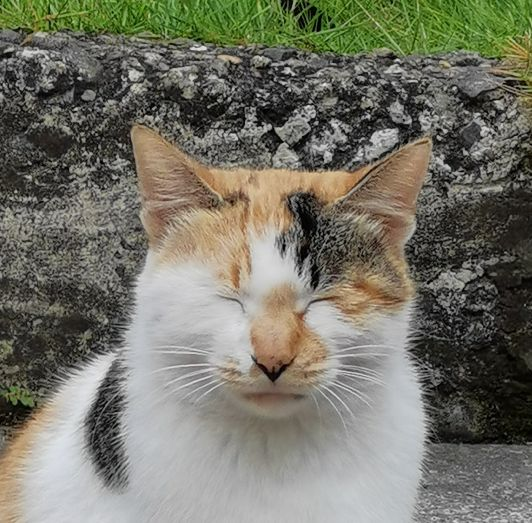
\includegraphics[scale=0.35]{pic1.jpg}
            }
            \subfigure[黑白图]
            {
                \centering
                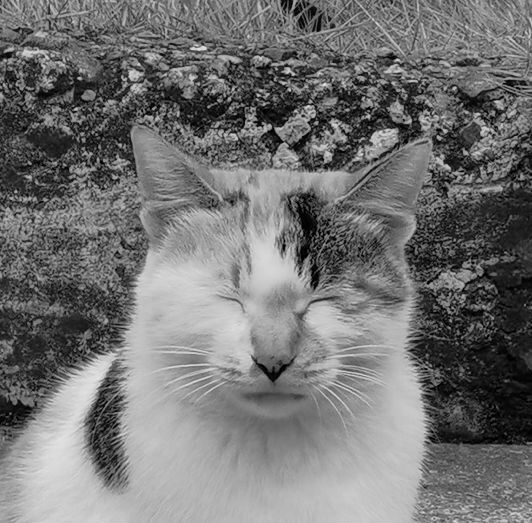
\includegraphics[scale=0.35]{pic1-黑白.jpg}
            }
        \end{center}
        \caption{广知B楼东门前空地上的三花猫(摄于2020年10月19日,命名为{\ttfamily pic1.jpg})}
        \label{cat}
    \end{figure}

    图(\ref{cat})颜色丰富,猫咪面部毛发浓密,背景有绿化与砖石,适合用来模糊后还原的比较。
    \begin{figure}[htbp]
        \begin{center}
            \subfigure[原图]
            {
                \centering
                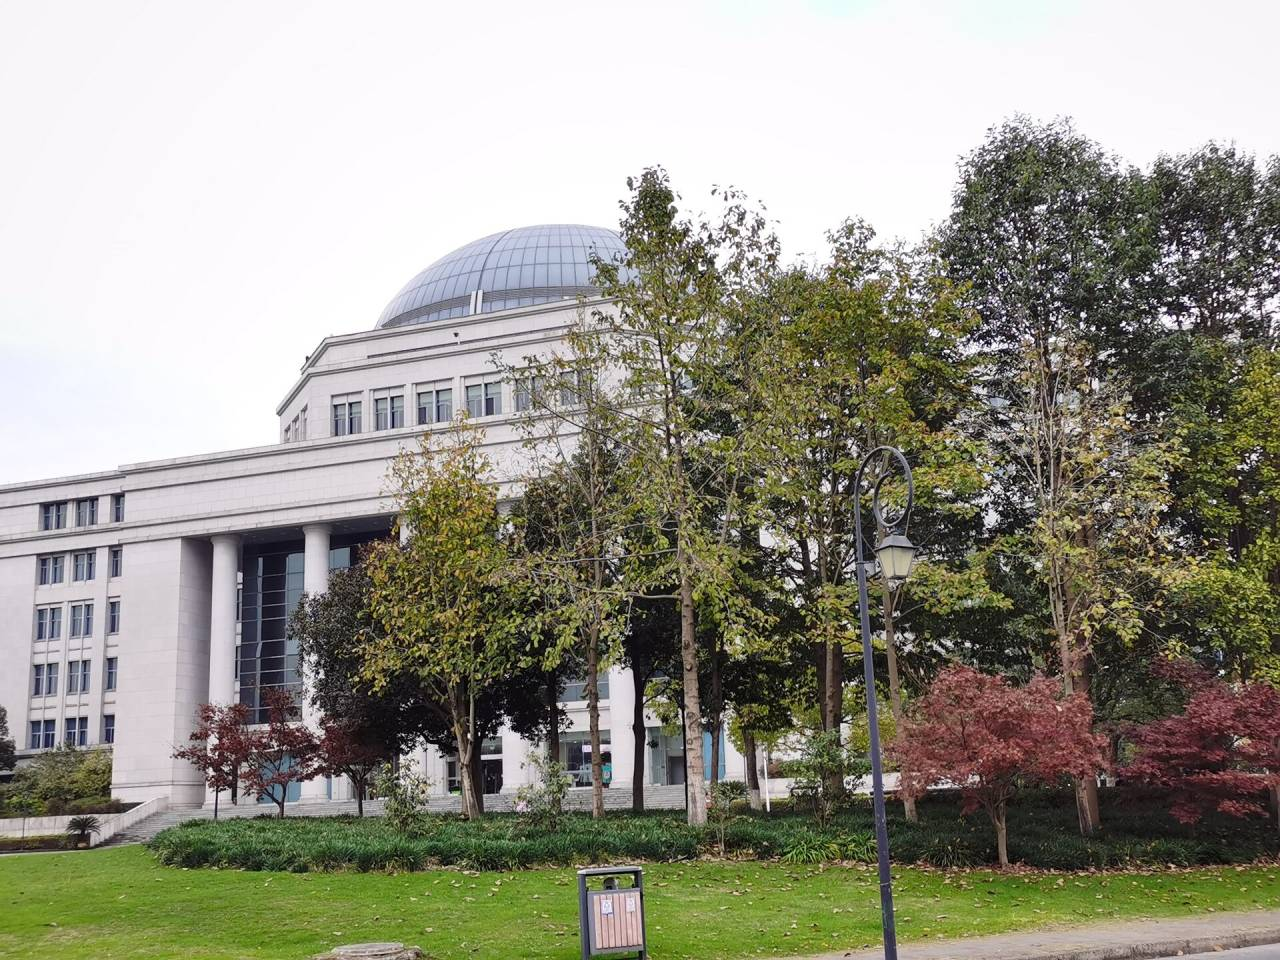
\includegraphics[scale=0.18]{pic2.jpg}
            }
            \subfigure[黑白图]
            {
                \centering
                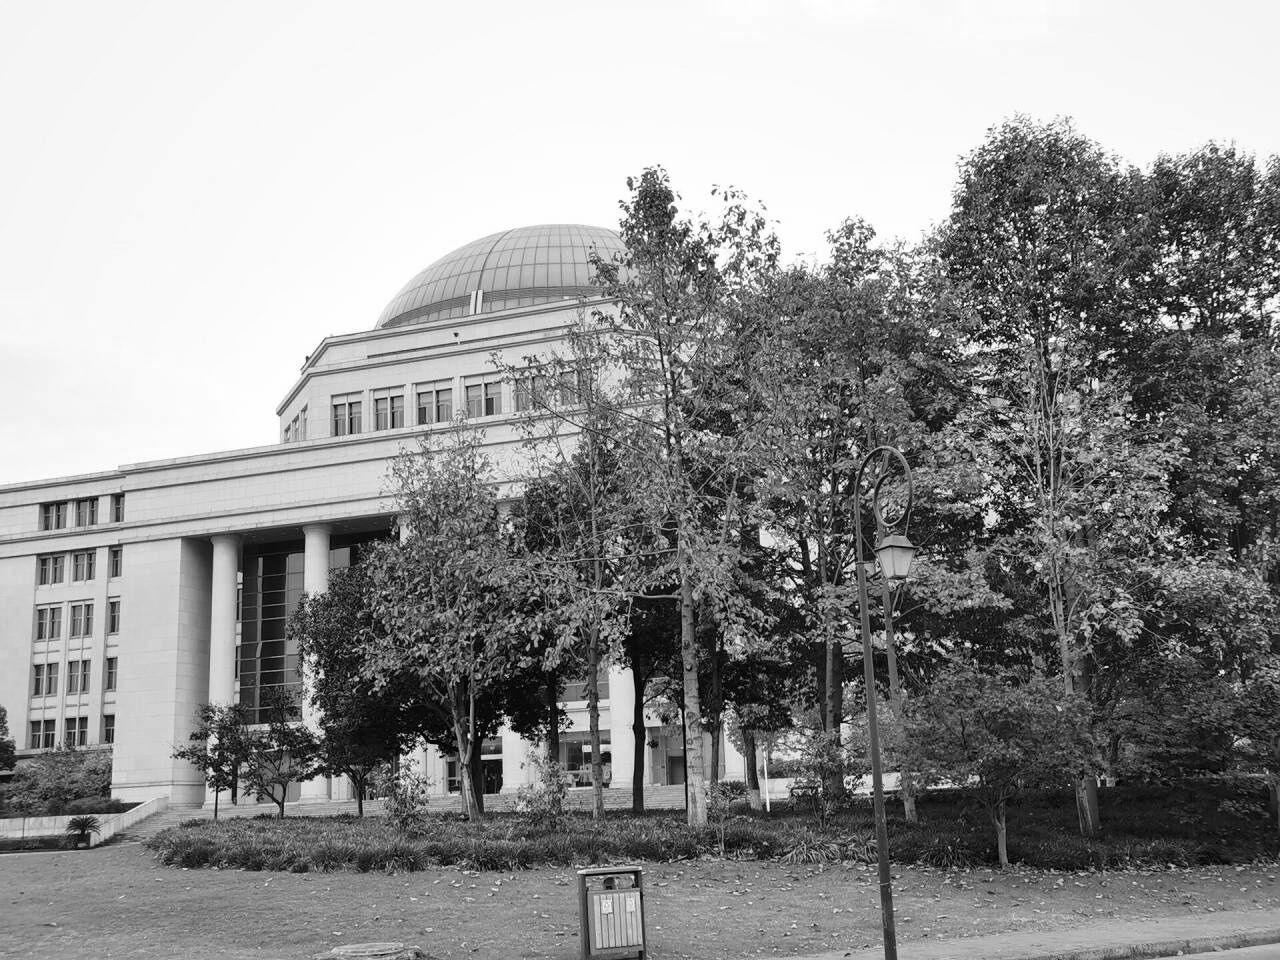
\includegraphics[scale=0.18]{pic2-黑白.jpg}
            }
        \end{center}
        \caption{图书馆大门西南角度(摄于2020年11月17日,命名为{\ttfamily pic2.jpg})}
        \label{library}
    \end{figure}

    图(\ref{library})颜色丰富,右半部分为绿化,细节颇多,左半部分是图书馆建筑,建筑宏大,整体线条形状明显,适合用来模糊后还原的比较。

    维纳滤波和约束最小二乘方滤波作为较常用的图像处理方法,在Matlab中提供了可以直接调用的函数,且使用起来相较其他语言(如Python,C,C++,VB等)更为简单,故本文选择Matlab进行介绍。维纳滤波有{\ttfamily deconvwnr}和{\ttfamily wiener2}函数等,约束最小二乘方滤波有{\ttfamily deconvreg}函数等。

    下文先介绍不直接调用Matlab所提供函数的方法,再介绍如何使用所提供的函数的方法,并简单对两种方法进行比较。
    \subsection{维纳滤波的Matlab代码与结果}
    \subsubsection{利用式(\ref{eqsetmin})对模糊加噪声图像进行维纳滤波复原}
    为方便理解,现将代码中部分用到的函数的作用放入下表做简单介绍:
    \begin{table}[htbp]
        \begin{center}
        \caption{对模糊加噪声图像进行维纳滤波复原代码中函数的介绍}
        \begin{tabular}{|c|c|}
            \hline
            函数 & 作用 \\ \hline
            {\ttfamily imread(filename.fmt)} & \tabincell{c}{根据文件名{\ttfamily filename}读取灰度获彩色图像,\\返回的是包含图像数据的数组}\\ \hline
            {\ttfamily rgb2gray(RGB)} & \tabincell{c}{消除图像色调和饱和度信息同时保留亮度\\将{\ttfamily RGB}图像或彩色图转换为灰度图像}\\ \hline
            {\ttfamily im2double(I)} & 将灰度图像{\ttfamily I}转换为双精度\\ \hline
            {\ttfamily size(A)} & 获取矩阵{\ttfamily \textit{A}}的行数和列数\\ \hline
            {\ttfamily fspecial(type, para)} & \tabincell{c}{用于建立预定义的滤波算子,\\其中{\ttfamily type}指定算子的类型,{\ttfamily para}指定相应的参数}\\ \hline
            {\ttfamily conv2(A,B)} & 计算矩阵{\ttfamily \textit{A}}和{\ttfamily \textit{B}}的卷积\\ \hline
            {\ttfamily zeros(m,n)} & 产生{\ttfamily \textit{m}}$\times${\ttfamily \textit{n}}的零矩阵\\ \hline
            {\ttfamily imnoise(f,type,parameters)} & \tabincell{c}{给一幅图像添加噪声,{\ttfamily f}是原图像,{\ttfamily type}是加入的噪声类型,\\{\ttfamily parameters}是噪声的一些参数}\\ \hline
            {\ttfamily figure} & 创建一个新的窗口,所有参数采用默认\\ \hline
            {\ttfamily imshow(I)} & 显示灰度图像{\ttfamily I}\\ \hline
            {\ttfamily title('caption')} & 设置图像的标题{\ttfamily caption}\\ \hline
            {\ttfamily fft2(X)} & 使用快速傅里叶变换算法返回矩阵{\ttfamily \textit{X}}的二维傅里叶变换\\ \hline
            {\ttfamily fftshift(X)} & 移动零频点到频谱中间,重新排列{\ttfamily fft}、{\ttfamily fft2}和{\ttfamily fftn}的输出结果\\ \hline
            {\ttfamily conj(Z)} & 返回{\ttfamily \textit{Z}}的元素的复共轭\\ \hline
            {\ttfamily ifftshift(X)} & 按负方向(向左和向上)做圆周位移\\ \hline
            {\ttfamily ifft2(Y)} & 使用快速傅里叶变换算法返回矩阵{\ttfamily \textit{Y}}的二维离散傅里叶逆变换\\ \hline
        \end{tabular}
    \end{center}
    \end{table}
    \clearpage
    代码如下:
    \begin{lstlisting}
% 使用另一张图只需将pic1.jpg改为pic2.jpg即可
Image=im2double(rgb2gray(imread('pic1.jpg')));
window=15;
[n, m]=size(Image);
n=n+window-1;
m=m+window-1;
% 点扩散函数
h=fspecial('average', window);
BlurredI=conv2(h, Image);
% 噪声信号
noise=imnoise(zeros(n, m),'salt & pepper', 0.001);
% 给模糊图像添加椒盐噪声
BlurrednoisyI=BlurredI+noise;
figure, imshow(BlurrednoisyI), title('Blurred Image with noise');
% 模板延拓
h1=zeros(n, m);
h1(1:window, 1:window)=h;
H=fftshift(fft2(h1));
% 计算信噪比
K=sum(noise(:).^2)/sum(Image(:).^2);
% 计算维纳滤波传递函数
M=conj(H)./(abs(H).^2+K);
G=fftshift(fft2(BlurrednoisyI));
f=ifft2(ifftshift(G.*M));
result=f(1:n-window+1, 1:m-window+1);
figure, imshow(abs(result), []), title('Filtered Image');
    \end{lstlisting}
    \clearpage
    对图(\ref{cat})的代码运行结果如下:
    \begin{figure}[htbp]
        \centering
        \subfigure[加噪声的模糊图像]
        {
            \centering
            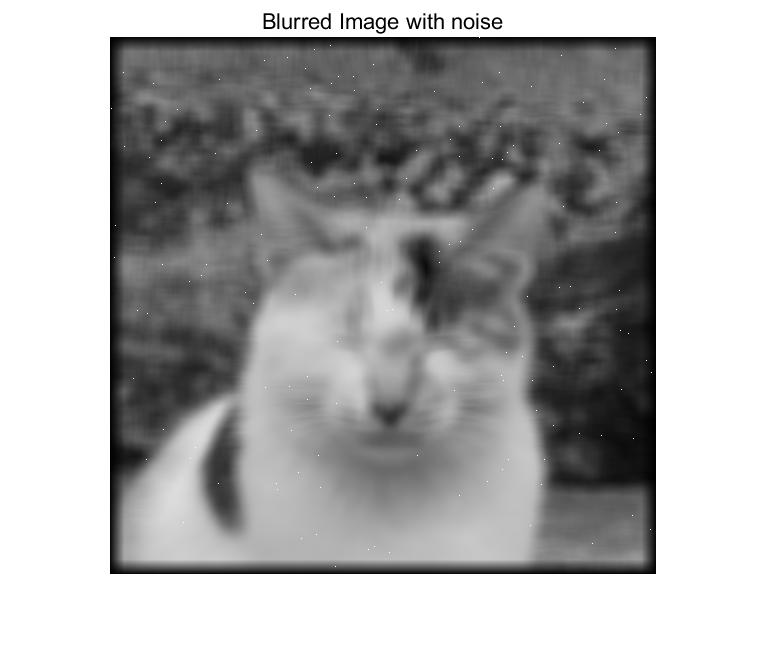
\includegraphics[scale=0.31]{pic1-2.2.1-1.jpg}
        }
        \subfigure[维纳滤波结果图像]
        {
            \centering
            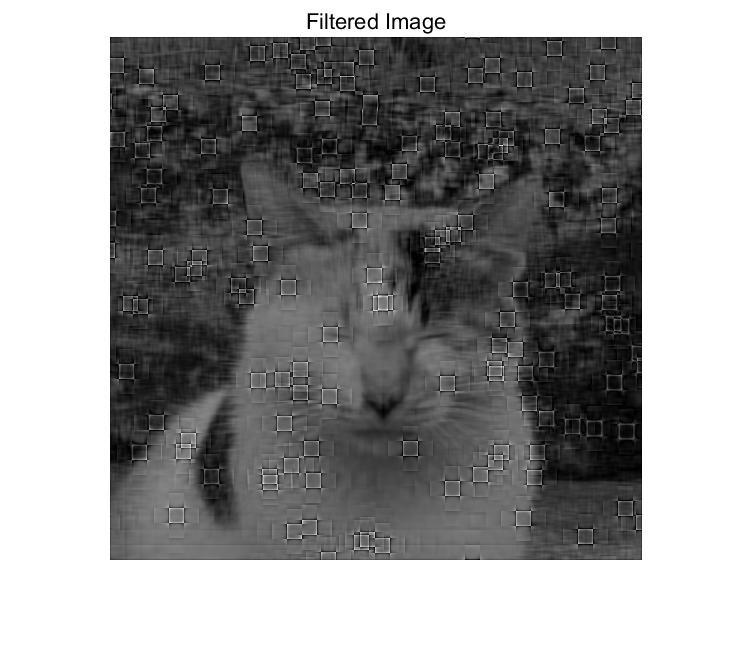
\includegraphics[scale=0.32]{pic1-2.2.1-2.jpg}
        }
        \caption{图(\ref{cat})的维纳滤波效果}
        \label{catweina1}
    \end{figure}

    对图(\ref{library})的代码运行结果如下(运行时只需将程序第一行的{\ttfamily pic1.jpg}改为{\ttfamily pic2.jpg}即可):
    \begin{figure}[htbp]
        \centering
        \subfigure[加噪声的模糊图像]
        {
            \centering
            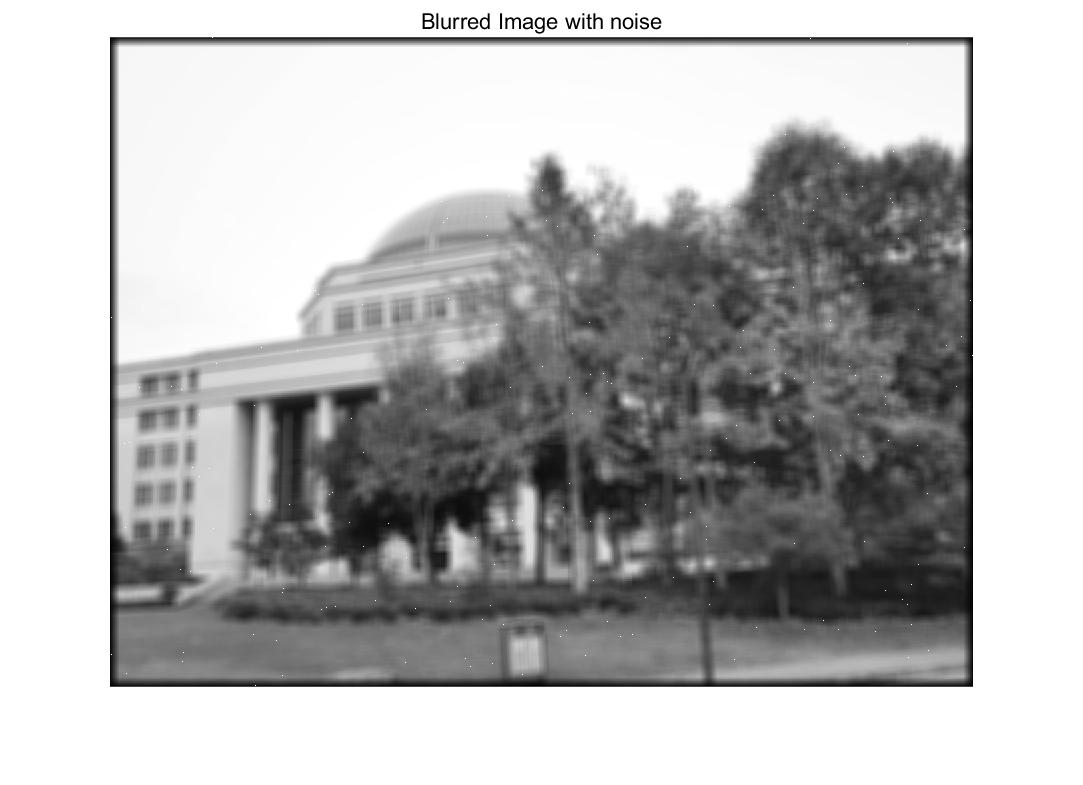
\includegraphics[scale=0.22]{pic2-2.2.1-1.jpg}
        }
        \subfigure[维纳滤波结果图像]
        {
            \centering
            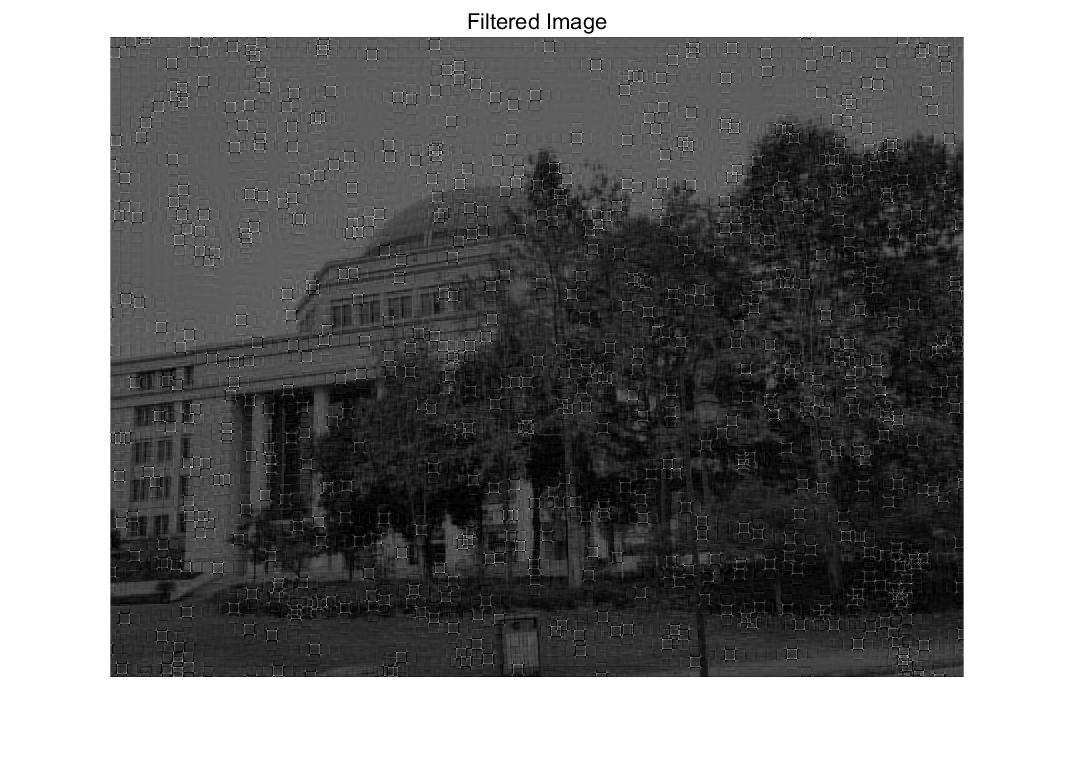
\includegraphics[scale=0.22]{pic2-2.2.1-2.jpg}
        }
        \caption{图(\ref{library})的维纳滤波效果}
        \label{libraryweina1}
    \end{figure}

    结果分析会在第三部分中进行说明。
    \clearpage
    \subsubsection{采用Matlab提供的函数,对运动模糊的图像进行维纳滤波}
    先介绍一下Matlab提供的进行维纳滤波的函数。
    \begin{enumerate}[label=(\arabic*),itemindent=1.5em]
        \item {\ttfamily deconvwnr}函数:使用维纳滤波器对图像进行去模糊。
        \begin{enumerate}[itemindent=1em]
            \item {\ttfamily J=deconvwnr(I,PSF)}:
            \par\setlength\parindent{1em}{\ttfamily PSF}为矩阵,表示点扩散函数。
            \item {\ttfamily J=deconvwnr(I,PSF,NSR)}:
            \par\setlength\parindent{1em}{\ttfamily NSR}为标量,表示信噪比,默认为{\ttfamily 0}。
            \item {\ttfamily J=deconvwnr(I,PSF,NCORR,ICORR)}:
            \par\setlength\parindent{1em}{\ttfamily NCORR}和{\ttfamily ICORR}为矩阵,分别表示噪声和原始图像的自相关函数值。
        \end{enumerate}
        \item {\ttfamily wiener2}函数:使用二维维纳滤波对图像进行降噪处理。
        \begin{enumerate}[itemindent=1em]
            \item {\ttfamily J=wiener2(I,[m n],noise)}:
            \par\setlength\parindent{1em}{\ttfamily m,n}为标量,指定{\ttfamily m}$\times${\ttfamily n}邻域估计图像均值和方差,默认$3\times3$;{\ttfamily noise}为矩阵,表示指定噪声。
            \item {\ttfamily [J,noise]=wiener2(I,[m n])}:
            \par\setlength\parindent{1em}降噪处理,并返回函数的估计噪声{\ttfamily noise}。
        \end{enumerate}
    \end{enumerate}

    在本段代码中只需额外再介绍一种Matlab的内置函数:
    \begin{table}[htbp]
        \begin{center}
        \caption{对运动模糊的图像进行维纳滤波中函数的介绍}
        \begin{tabular}{|c|c|}
            \hline
            函数 & 作用 \\ \hline
            {\ttfamily imfilter(f,w,fm,bo,so)} & \tabincell{c}{对任意类型数组或多维图像进行滤波,\\{\ttfamily f}是输入图像,{\ttfamily w}为滤波模板,{\ttfamily g}为滤波结果,\\{\ttfamily fm}为滤波模式,{\ttfamily bo}为边界选项,{\ttfamily so}为大小选项} \\ \hline
        \end{tabular}
        \end{center}
    \end{table}
    \clearpage
    代码如下:
    \begin{lstlisting}
% 使用另一张图只需将pic1.jpg改为pic2.jpg即可
Image=im2double(rgb2gray(imread('pic1.jpg')));
% 运动模糊参数,11°方向上移21个像素
LEN=21;
THETA=11;
% 点扩散函数
PSF=fspecial('motion', LEN, THETA);
% 产生模糊图像
BlurredI=imfilter(Image, PSF, 'conv', 'circular');
% 噪声参数
noise_mean=0;
noise_var=0.0001;
% 生成模糊加噪声图像
BlurrednoisyI=imnoise(BlurredI, 'gaussian', noise_mean, noise_var);
figure, imshow(BlurrednoisyI), title('Simulate Blur and Noise');
% 估计信噪比为0
estimated_nsr=0;
% 维纳滤波去模糊
result1=deconvwnr(BlurrednoisyI, PSF, estimated_nsr);
figure, imshow(result1), title('Restoration Using NSR=0');
% 设置信噪比为噪声与图像方差比
estimated_nsr=noise_var/var(Image(:));
% 维纳滤波去模糊
result2=deconvwnr(BlurrednoisyI, PSF, estimated_nsr);
figure, imshow(result2), title('Restoration Using Estimated NSR');
    \end{lstlisting}
    \clearpage
    对图(\ref{cat})的代码运行结果如下:
    \begin{figure}[htbp]
        \centering
        \subfigure[运动模糊加高斯噪声图像]
        {
            \centering
            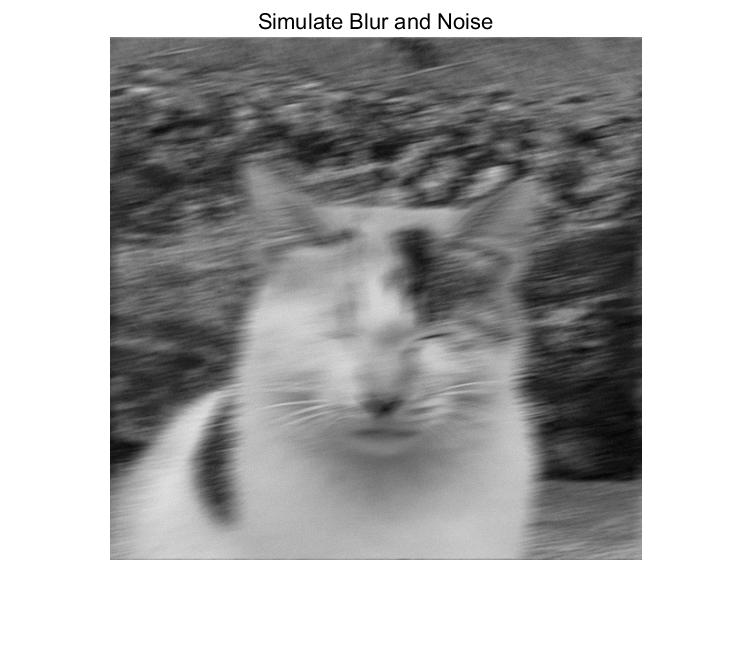
\includegraphics[scale=0.31]{pic1-2.2.2-1.jpg}
        }
        \subfigure[维纳滤波复原($\text{NSR}=0$)]
        {
            \centering
            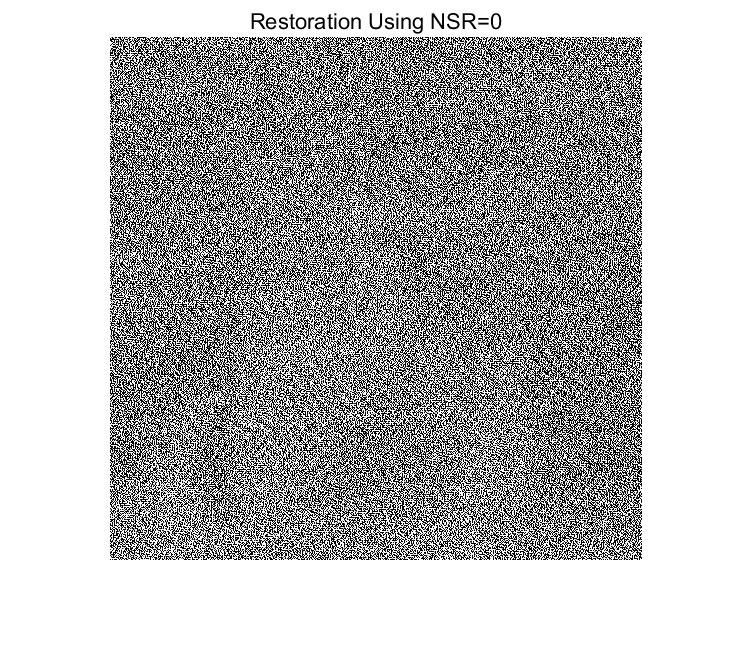
\includegraphics[scale=0.31]{pic1-2.2.2-2.jpg}
        }
        \subfigure[维纳滤波复原(估计NSR)]
        {
            \centering
            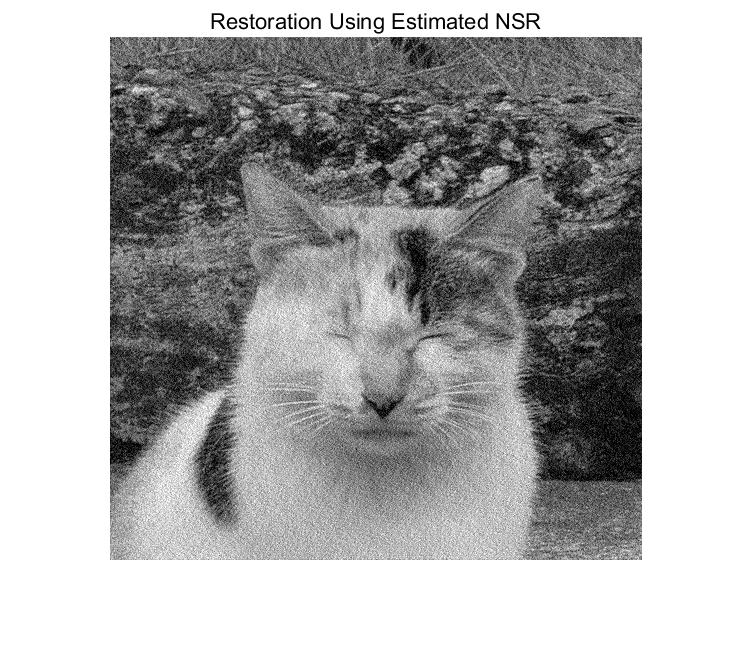
\includegraphics[scale=0.31]{pic1-2.2.2-3.jpg}
        }
        \caption{图(\ref{cat})的维纳滤波恢复运动模糊加高斯噪声图像}
        \label{catweina2}
    \end{figure}
    \clearpage
    对图(\ref{library})的代码运行结果如下(运行时只需将程序第一行的{\ttfamily pic1.jpg}改为{\ttfamily pic2.jpg}即可):
    \begin{figure}[htbp]
        \centering
        \subfigure[运动模糊加高斯噪声图像]
        {
            \centering
            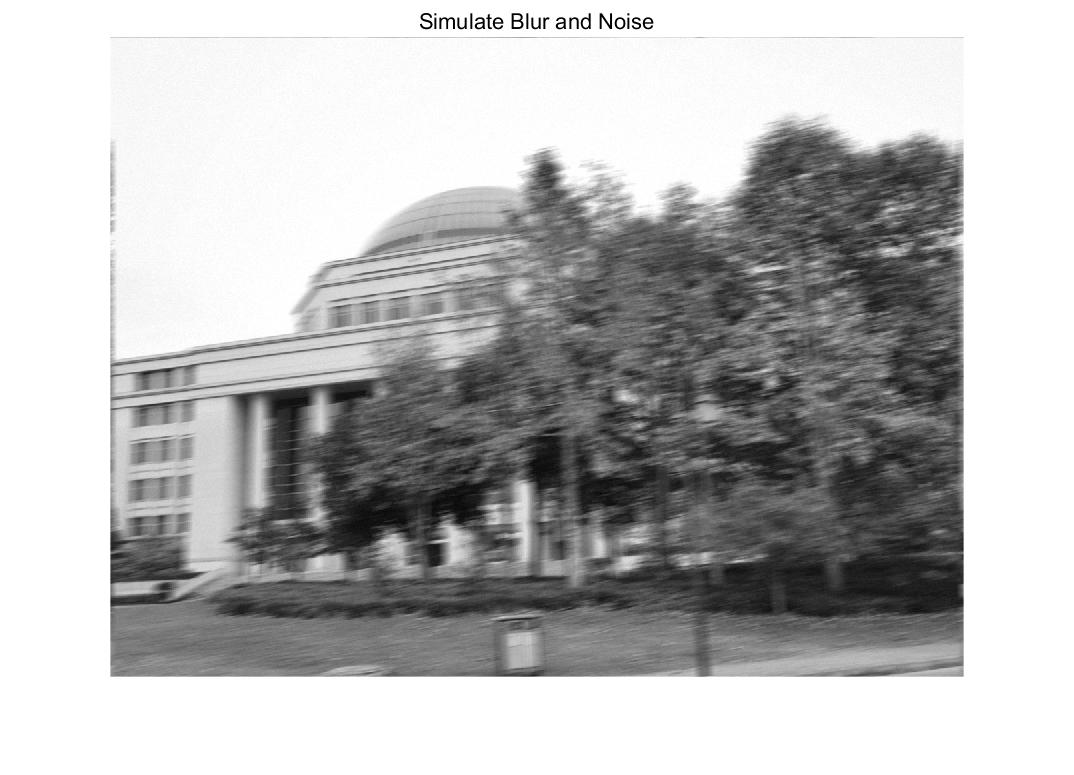
\includegraphics[scale=0.22]{pic2-2.2.2-1.jpg}
        }
        \subfigure[维纳滤波复原($\text{NSR}=0$)]
        {
            \centering
            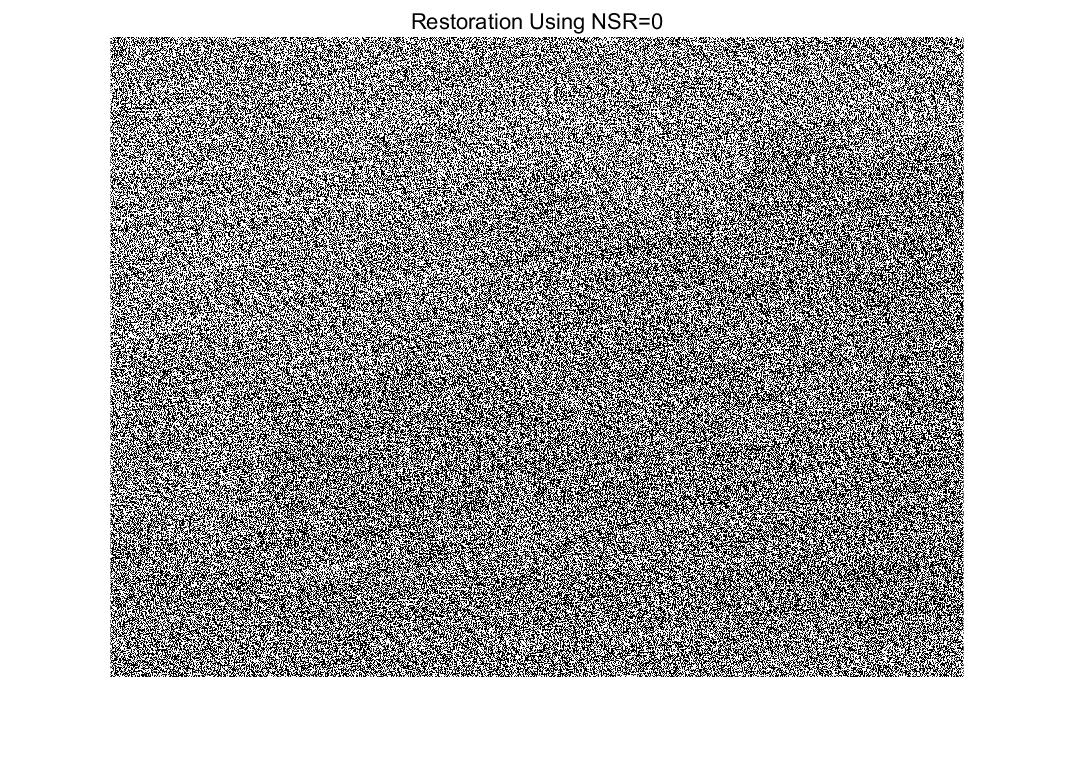
\includegraphics[scale=0.22]{pic2-2.2.2-2.jpg}
        }
        \subfigure[维纳滤波复原(估计NSR)]
        {
            \centering
            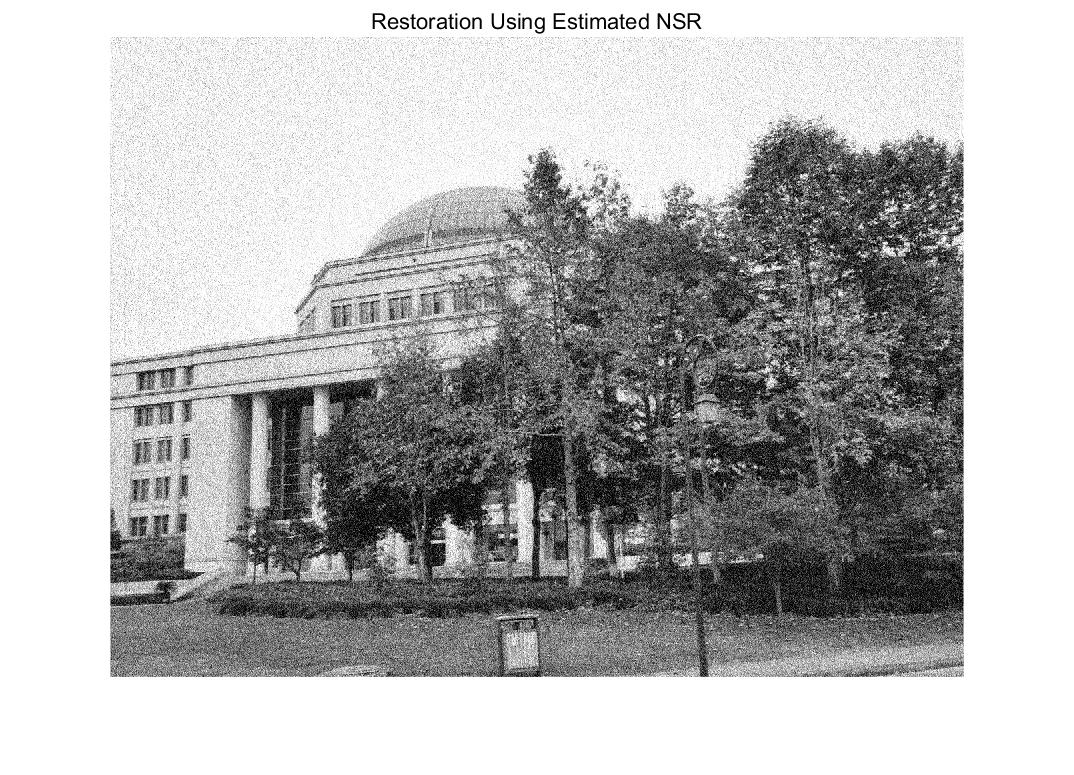
\includegraphics[scale=0.22]{pic2-2.2.2-3.jpg}
        }
        \caption{图(\ref{library})的维纳滤波恢复运动模糊加高斯噪声图像}
        \label{libraryweina2}
    \end{figure}

    结果分析会在第三部分中进行说明。
    \subsection{约束最小二乘方滤波的Matlab代码与结果}
    \subsubsection{对模糊的图像进行约束最小二乘方滤波}
    下方代码中所出现的Matlab的内置函数在介绍维纳滤波时已经介绍过了,这里不再赘述。
    \clearpage
    \begin{lstlisting}
% 使用另一张图只需将pic1.jpg改为pic2.jpg即可
Image=im2double(rgb2gray(imread('pic1.jpg')));
window=15; [N, M]=size(Image);
N=N+window-1; M=M+window-1;
h=fspecial('average', window); % 点扩散函数
BlurredI=conv2(h, Image); % 图像模糊
sigma=0.001; miun=0; % 噪声的方差、均值参数
nn=M*N*(sigma+miun*miun); % 约束值
BlurrednoisyI=imnoise(BlurredI, 'gaussian', miun, sigma); % 模糊加噪声图像
figure, imshow(BlurrednoisyI), title('Blurred Image with noise');
h1=zeros(N, M); h1(1:window, 1:window)=h; % 点扩散函数延拓
H=fftshift(fft2(h1)); % 频域退化函数
lap=[0 1 0; 1 -4 1; 0 1 0]; % 二阶微分模板
L=zeros(N, M); L(1:3, 1:3)=lap; % 微分模板延拓
L=fftshift(fft2(L)); % 频域微分模板
G=fftshift(fft2(BlurrednoisyI)); % 退化函数DFT
gama=0.3; step=0.01; alpha=nn*0.001; % 初始γ值、γ修正步长、准确度系数
flag=true; % 循环标识变量
while flag
    MH=conj(H)./abs(H).^2+gama*(abs(L).^2); % 估计复原函数
    F=G.*MH; E=G-H.*F;
E=abs(ifft2(ifftshift(E))); ee=sum(E(:).^2); % 复原图像并计算残差
    if ee<nn-alpha % 判断并修正γ值
        gama=gama+step;
    elseif ee>nn+alpha
        gama=gama-step;
    else
        flag=false;
    end
end
MH=conj(H)./(abs(H).^2+gama*(abs(L).^2)); % 计算最终复原函数
f=ifft2(ifftshift(G.*MH));
result=f(1:N-window+1, 1:M-window+1); % 复原图像
figure, imshow(abs(result), []), title('Filtered Image');
    \end{lstlisting}
    \clearpage
    对图(\ref{cat})的代码运行结果如下:
    \begin{figure}[htbp]
        \centering
        \subfigure[模糊加高斯噪声图像]
        {
            \centering
            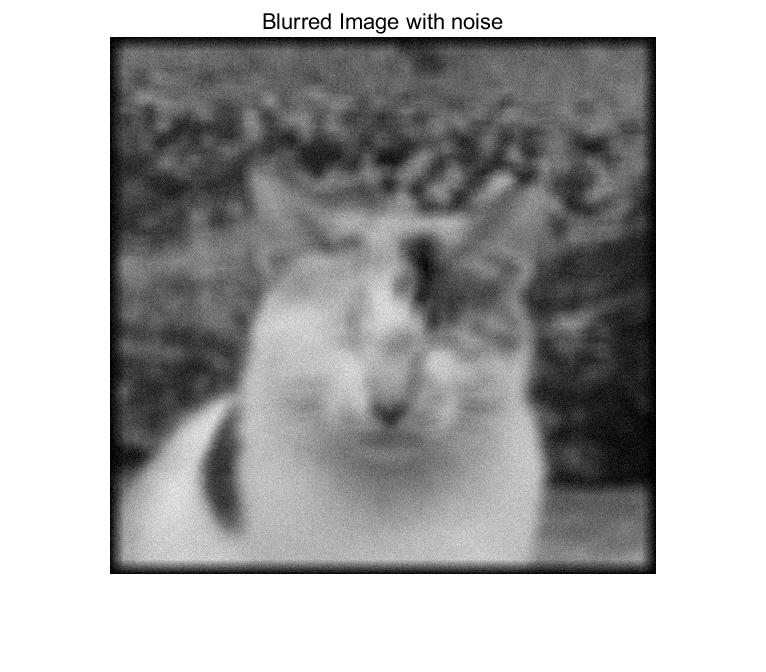
\includegraphics[scale=0.31]{pic1-2.3.1-1.jpg}
        }
        \subfigure[约束最小二乘方滤波]
        {
            \centering
            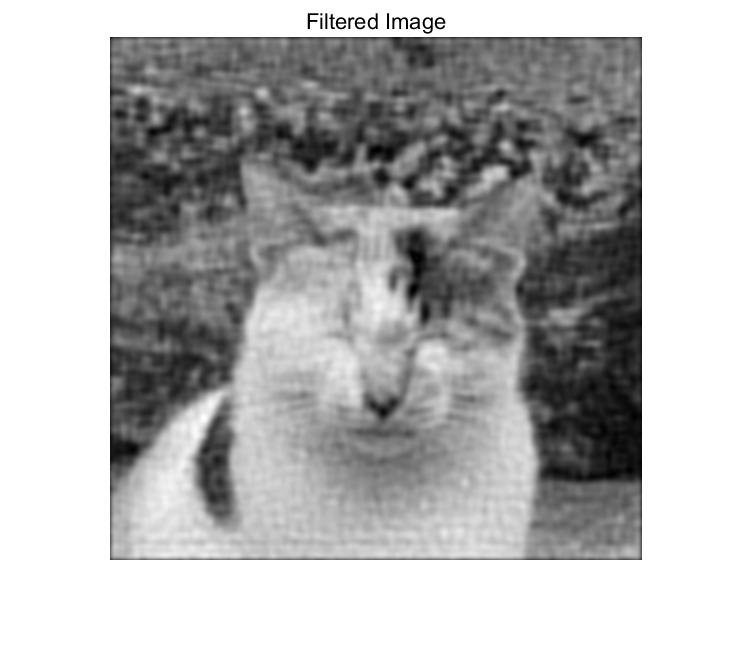
\includegraphics[scale=0.31]{pic1-2.3.1-2.jpg}
        }
        \caption{图(\ref{cat})的约束最小二乘方滤波效果示意图}
        \label{catlimitmin1}
    \end{figure}

    对图(\ref{library})的代码运行结果如下:
    \begin{figure}[htbp]
        \centering
        \subfigure[模糊加高斯噪声图像]
        {
            \centering
            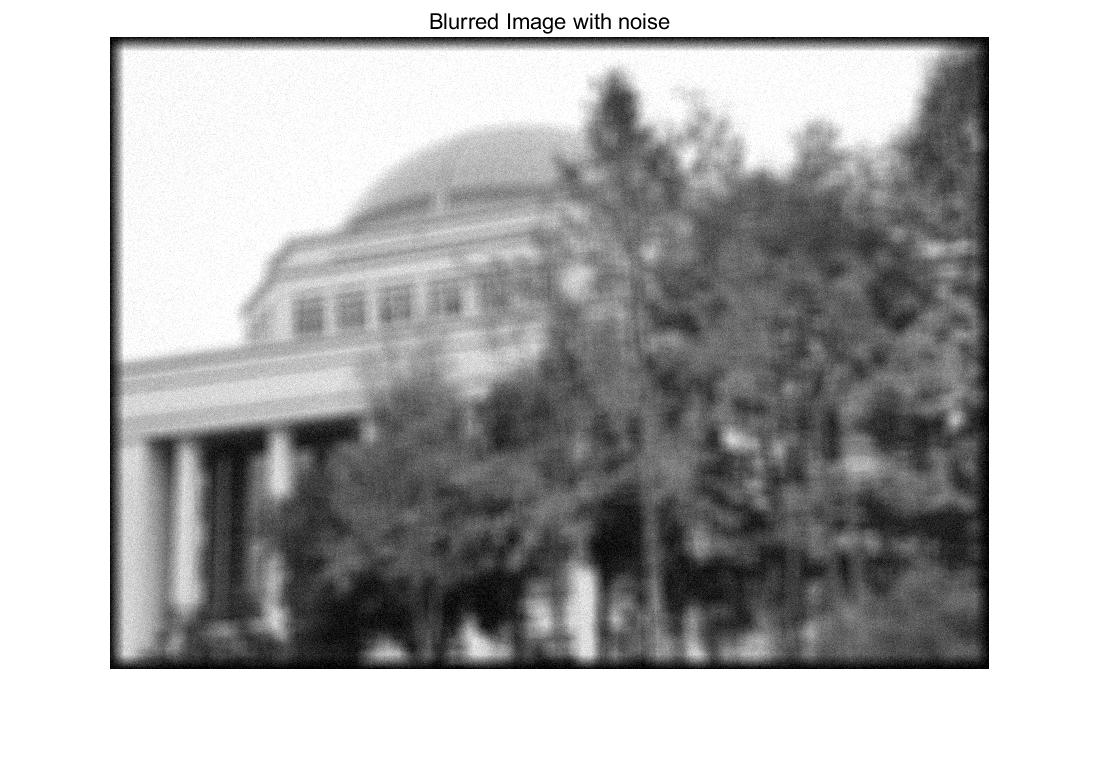
\includegraphics[scale=0.22]{pic2-2.3.1-1.jpg}
        }
        \subfigure[约束最小二乘方滤波]
        {
            \centering
            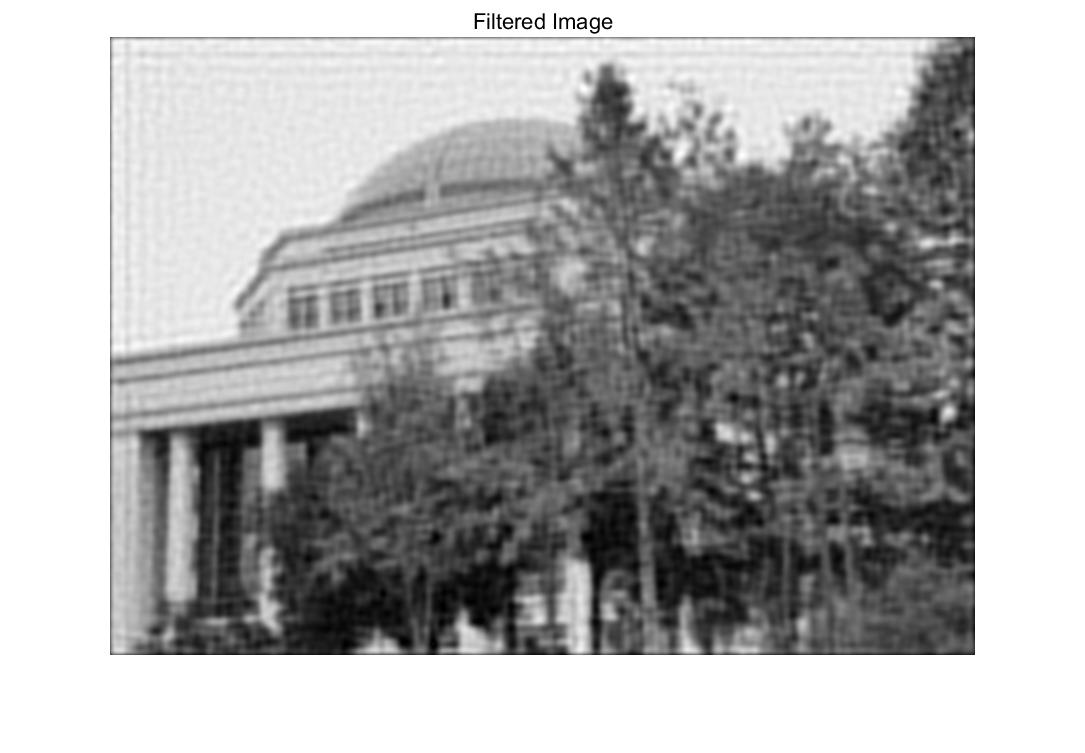
\includegraphics[scale=0.22]{pic2-2.3.1-2.jpg}
        }
        \caption{图(\ref{library})的约束最小二乘方滤波效果示意图}
        \label{librarylimitmin1}
    \end{figure}

    由于图(\ref{library})尺寸过大,使用其局部进行约束最小二乘方滤波图像处理(下一节也是这样)。结果分析会在第三部分中进行说明。
    \subsubsection{利用Matlab内置函数进行约束最小二乘方滤波图像处理}
    先介绍一下Matlab提供的进行约束最小二乘方滤波的函数{\ttfamily deconvreg}。
    \begin{enumerate}[label=(\arabic*),itemindent=1.5em]
        \item {\ttfamily J=deconvwnr(I,PSF,NP)}
        \item {\ttfamily J=deconvwnr(I,PSF,NP,LRANGE)}
        \item {\ttfamily J=deconvwnr(I,PSF,NP,LRANGE,REGOP)}
        \item {\ttfamily [J,LAGRA]=deconvwnr(I,PSF,$\cdots$)}
    \end{enumerate}

    参数含义:

    {\ttfamily I}:降质图像;{\ttfamily J}:复原图像;{\ttfamily PSF}:退化过程的点扩散函数;{\ttfamily NP}:加性噪声能量,默认值为{\ttfamily 0};{\ttfamily LRANGE}:拉格朗日乘子系数的优化范围,默认值为$[10^{-9},10^9]$;{\ttfamily REGOP}:去卷积的线性约束算子,默认时为二维拉普拉斯算子。{\ttfamily LAGRA}为计算出的最优拉格朗日乘子系数。

    调用{\ttfamily deconvreg}函数时只需要在上方代码中稍微修改即可。代码如下:
    \begin{lstlisting}
% 前面部分代码与上方代码中的1到33行一致
J=deconvreg(BlurrednoisyI, h, nn);
figure, imshow(J, []), title('Filtered Image');
    \end{lstlisting}

    对图(\ref{cat})的代码运行结果如下:
    \begin{figure}[htbp]
        \centering
        \subfigure[模糊加高斯噪声图像]
        {
            \centering
            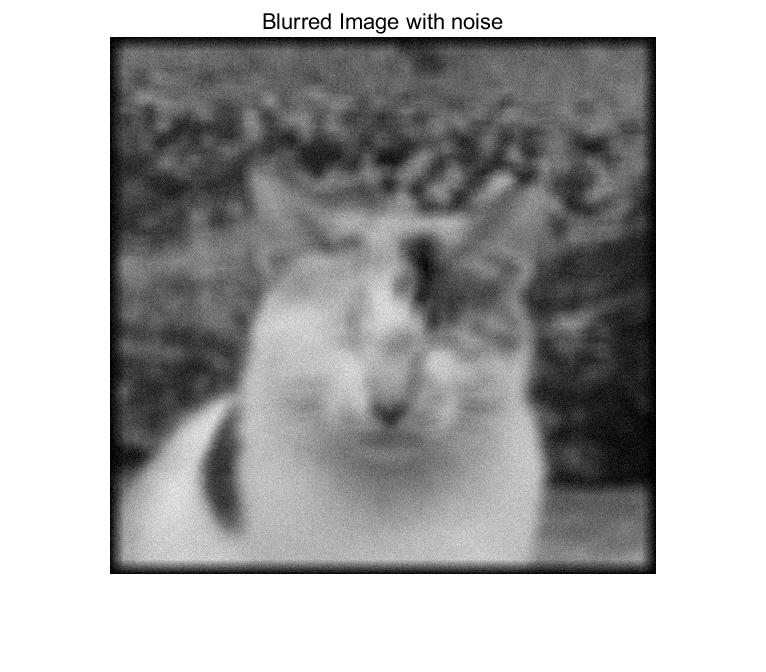
\includegraphics[scale=0.31]{pic1-2.3.2-1.jpg}
        }
        \subfigure[约束最小二乘方滤波]
        {
            \centering
            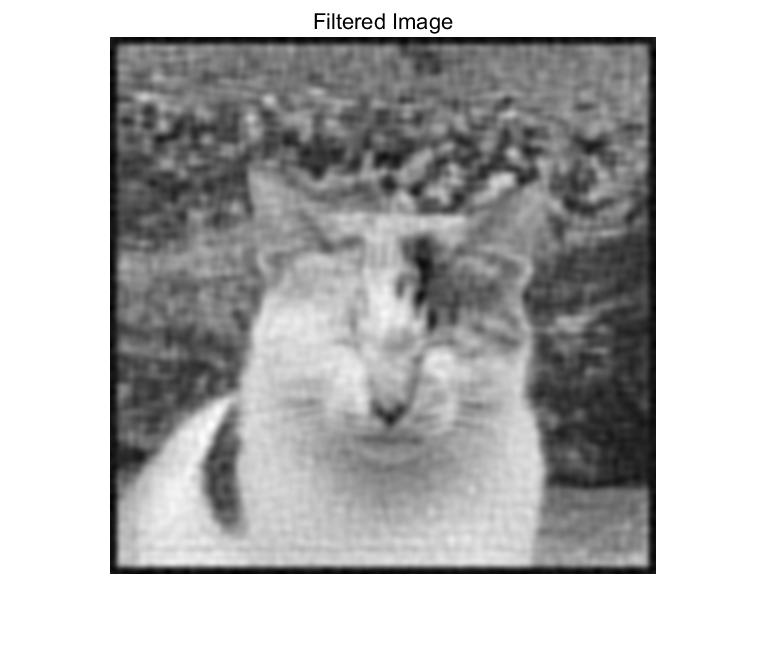
\includegraphics[scale=0.31]{pic1-2.3.2-2.jpg}
        }
        \caption{图(\ref{cat})的约束最小二乘方滤波效果示意图}
        \label{catlimitmin2}
    \end{figure}
    \clearpage
    对图(\ref{library})的代码运行结果如下:
    \begin{figure}[htbp]
        \centering
        \subfigure[模糊加高斯噪声图像]
        {
            \centering
            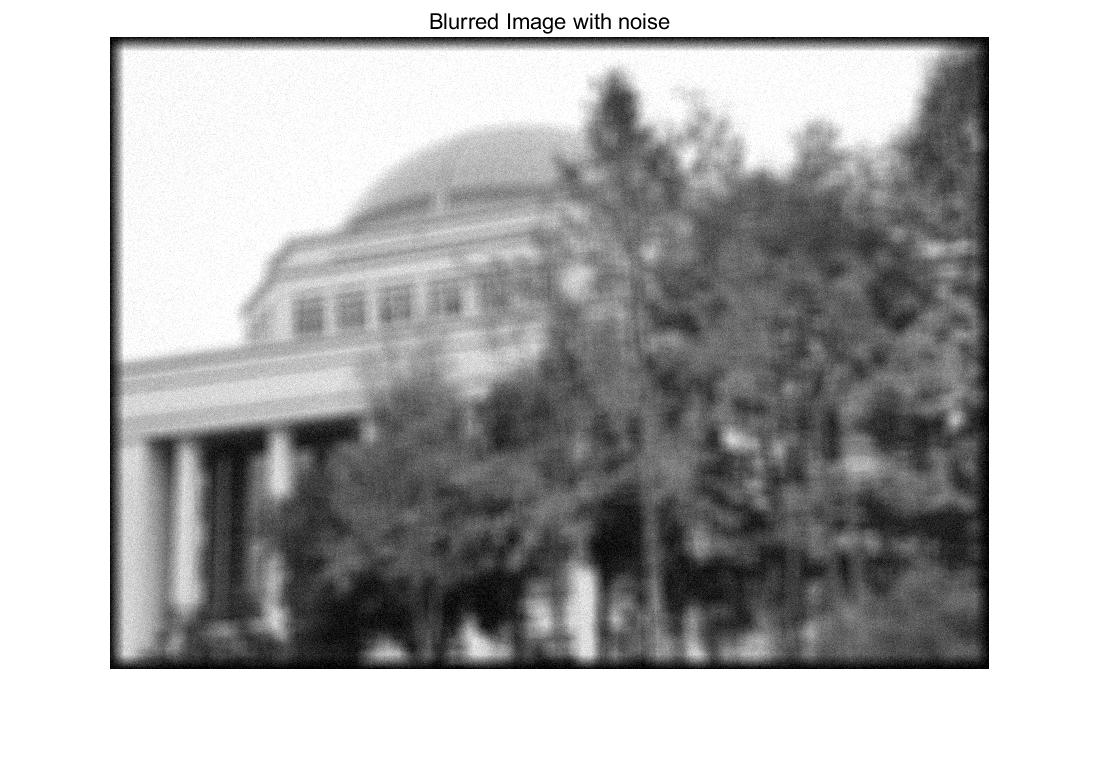
\includegraphics[scale=0.22]{pic2-2.3.1-1.jpg}
        }
        \subfigure[约束最小二乘方滤波]
        {
            \centering
            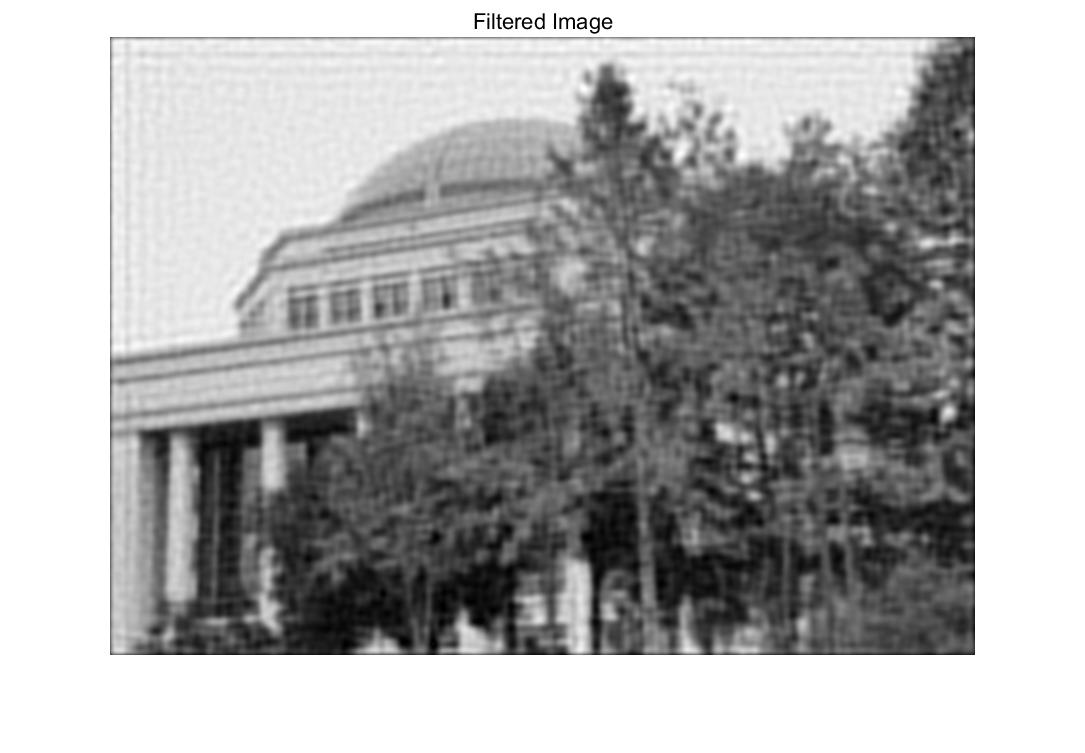
\includegraphics[scale=0.22]{pic2-2.3.1-2.jpg}
        }
        \caption{图(\ref{library})的约束最小二乘方滤波效果示意图}
        \label{librarylimitmin2}
    \end{figure}

    由于图(\ref{library})尺寸过大,使用其局部进行约束最小二乘方滤波图像处理。结果分析会在第三部分中进行说明。
    \section{两种图像复原结果分析与比较}
    \subsection{维纳滤波结果分析}
    \subsubsection{利用式(\ref{eqsetmin})对模糊加噪声图像进行维纳滤波复原分析}
    在程序中添加了$15 \times 15$的均值滤波,添加了同样密度的椒盐噪声,在仅观察被添加了椒盐噪声和经过维纳滤波复原的两张图时能看出,维纳滤波确实在一定程度上复原了图片的本来面貌,但是可以发现,经过了维纳滤波图像复原的图片表面出现了波纹,与最希望得到的结果(即复原成原图或原图的黑白模式)相差较远。

    同时由于程序中已知噪声和退化函数,能够计算信噪比$K$,而在实际问题中需要人为地去估计$K$的值。因此,我们可以用Matlab中内置的关于维纳滤波的函数进行处理,效果相较来说会比图(\ref{catweina1})好。
    \subsubsection{采用Matlab提供的函数,对运动模糊的图像进行维纳滤波的分析}
    根据图(\ref{catweina2})和图(\ref{libraryweina2})的结果可以看出,运用Matlab自带的维纳滤波函数比自己去编写具有类似功能的代码结果要好。图(\ref{catweina2})的图(c)中没有出现类似于图(\ref{catweina1})的图(b)中的波纹,同时其复原效果也确实比之前的更佳[明显地,图(\ref{libraryweina1})和图(\ref{libraryweina2})也有这样的结果],实际上当$\text{NSR}=0$时,维纳滤波就相当于是逆滤波,也很明显,仅仅运用逆滤波对加入了运动模糊和高斯噪声的图像的复原效果不佳,甚至没有复原出原图的任何特征。

    维纳滤波复原较逆滤波复原能够获得更好的效果。但是,正如在原理部分叙述的,维纳滤波需要知道原始图像和噪声的功率谱$S_f(u,v)$和$S_n(u,v)$,而实际上这些值是未知的,功率谱比的常数估计一般还是没有合适的解。若仅知道噪声方差的情况,可考虑约束最小二乘方滤波,也就引出了下一部分。
    \subsection{约束最小二乘方滤波结果分析}
    \subsubsection{对模糊的图像进行约束最小二乘方滤波}
    从图(\ref{catlimitmin1})中来看,其复原效果不算差,图(\ref{catlimitmin1})的图(a)十分模糊,边界线条很不清楚,但图(\ref{catlimitmin1})的图(b)对图(a)的复原总体不错,边界线条变得明显,整体变得明亮,复原效果还是很不错的。但是图上偏白的部分出现了小斑点。图(\ref{librarylimitmin1})和图(\ref{librarylimitmin2})也有类似结果。
    \subsubsection{利用Matlab内置函数进行约束最小二乘方滤波图像处理}
    利用Matlab内置函数进行约束最小二乘方滤波图像处理后,和用自己编写代码的结果类似,不过有一些细微的区别。图(\ref{catlimitmin2})的图(b)比图(\ref{catlimitmin1})的图(b)更加细腻,更加明亮。图(\ref{librarylimitmin1})和图(\ref{librarylimitmin2})也有类似结果。
    \subsection{两种图像处理方法比较分析}
    可以看出来,图(\ref{catweina2})中的图(c)比图(\ref{catlimitmin2})中的图(b)更加清楚,但也同样的经过程序模糊之后的图(\ref{catweina2})中的图(a)和图(\ref{catlimitmin2})中的图(a)也更加模糊,所以约束最小二乘方滤波和维纳滤波在不同的情况下也有不同的优势。

    不过也正如在维纳滤波中为引出约束最小二乘方滤波时所说的,约束最小二乘方滤波可以在条件较少的时候也可以进行图像的复原,否则维纳滤波则无法进行图像的复原。主要是因为维纳滤波建立在最小化统计准则的基础上,它所得到的结果只是平均意义上的最优,这使得约束最小二乘方滤波不会出现维纳滤波复原时无法复原的问题,对于所处理每一张图像都能产生最优的结果。实际上,在有的情况下,约束最小二乘方滤波的处理结果会比维纳滤波的结果要好,这是因选取的样本照片只有2张,较少,所以碰巧都没有出现这样的结果。

    \begin{thebibliography}{1}
        \bibitem{cai} 蔡利梅,王利娟. 数字图像处理. 徐州:中国矿业大学出版社, 2014.08.
        \bibitem{wu} 吴国平. 数字图像处理原理. 武汉:中国地质大学出版社, 2007.09.
    \end{thebibliography}
\end{document}